\documentclass[11pt]{article}

\usepackage[letterpaper, margin=1in]{geometry}

\usepackage[spanish]{babel}
\usepackage[utf8]{inputenc}
\usepackage{multirow}
\usepackage{tabularx}
\usepackage{longtable}



%Figuras
\usepackage{graphicx, subfigure}
\usepackage[]{tikz}
\usepackage{pbox}

%Matemática
\usepackage{amsmath}
\usepackage{amssymb}

%Símbolos mate extra (alfabetos, etc.)
\usepackage{mathrsfs}


%Algoritmos
\usepackage{float}
\usepackage{algorithm}
\usepackage{algorithmicx}
\usepackage{algpseudocode}
\usepackage{listings}


\usepackage{color}
\usepackage{hyperref}

\usepackage{mdframed}
\usepackage{tcolorbox}
\usepackage{multicol}
\usepackage{booktabs}
\usepackage{tabulary}
\definecolor{darkblue}{rgb}{0 , 0.054 , 0.196}



\title{Herencia- Pokemon}
\author{Leonardo Hern\'andez Chac\'on   - B43262}

\begin{document}

\maketitle
\hrule
\hrule
\tableofcontents
\hspace{5mm}
\hrule
\hrule


\section{Enunciado}

Implemente un programa en C++ utilizando herencia que modele las tres aves legendarias de Pokemon: Articuno, Moltres y Zapdos:

\begin{itemize}
\item Implemente una clase abstracta Pokemon que contenga:

    \begin{itemize}
    \item Atributos: name, species, HP, ATK, DEF, sATK, sDEF, SPD, EXP, call.  
    \item M\'etodos:
       \begin{itemize}
         \item virtual void atk1(Pokemon &other) = 0
         \item virtual void atk2(Pokemon &other) = 0
         \item virtual void atk3(Pokemon &other) = 0
         \item virtual void atk4(Pokemon &other) = 0
         \item string call()
         \item void printInfo()
       \end{itemize}
  
    \end{itemize}

\item Implemente cuatro clases llamadas Electric, Fire, Water y Flying que modelan los tipos de aves m\'iticas. Estas clases heredan de la clase Pokemon.
\begin{itemize}
\item M\'etodos
    \begin{itemize}
    \item static string type()
    \item static string strongVs()
    \item static string weakVs()
    \end{itemize}
\end{itemize}
  
\item Implemente tres clases concretas llamadas Zapdos, Articuno y Moltres.  
    \begin{itemize}
    \item Atributos
        \begin{itemize}
             \item Type, strongVs, weakVs
        \end{itemize}
    \item Metodos
        \begin{itemize}
             \item void print()
        \end{itemize}
    \end{itemize}
    
\item  Las clases  Zapdos, Articuno y Moltres deben implementar los m\'etodos virtuales puros y un m\'etodo que imprima el estado del pokemon con todos sus atributos. Haga un programa de prueba en donde se creen dos objetos e interactuen entre ellos(se ataquen un par de veces).  
    
\end{itemize}

\section{Desglose}
Se implementó las clases en programas como sigue:

\begin{itemize}
    \item Clase Pokemon
        \begin{itemize}
             \item Pokemon.cpp
             \item Pokemon.hpp
        \end{itemize}
    \item Clases Tipo
        \begin{itemize}
             \item Electric
                \begin{itemize}
                \item Electric.cpp
                \item Electric.hpp
                 \end{itemize}
             \item Water
                \begin{itemize}
                \item Water.cpp
                \item Water.hpp
                 \end{itemize}
             \item Fire
                \begin{itemize}
                \item Fire.cpp
                \item Fire.hpp
                 \end{itemize}
             \item Flying
             \begin{itemize}
                \item Flying.cpp
                \item Flying.hpp
                 \end{itemize}
                  \end{itemize}
    \item Clases Pokemones Legendarios  
        \begin{itemize}
                \item Zapdos
                    \begin{itemize}
                    \item Zapdos.cpp
                    \item Zapdos.hpp
                    \end{itemize}
                \item Moltres
                    \begin{itemize}
                    \item Moltres.cpp
                    \item Moltres.hpp
                    \end{itemize}
                \item Articuno
                    \begin{itemize}
                    \item Articuno.cpp
                    \item Articuno.hpp
                    \end{itemize}
        \end{itemize}
       
    
    \end{itemize}










\section{Pokemon}
\subsection{Pokemon.hpp}

\begin{lstlisting}[language=C]
#ifndef POKEMON_HPP
#define POKEMON_HPP

#include <iostream>

using namespace std;

class Pokemon {
public:
    Pokemon();
    virtual ~Pokemon();
   
    //Metodos
    void printInfo();
    string callPokemon();
    
    //Metodos virtuales puros, que estan implementados en una clase inferior
    virtual void atk1(Pokemon &other)=0;
    virtual void atk2(Pokemon &other)=0;
    virtual void atk3(Pokemon &other)=0;
    virtual void atk4(Pokemon &other)=0;

    //Atributos
    string name;
    string species;
    int life;
    int HP;
    int ATK;
    int DEF;
    int sATK;
    int sDEF;
    int SPD;
    int EXP;
    string call; 
   
};

#endif /* POKEMON_HPP */
\end{lstlisting}



\subsection{Pokemon.cpp}

\begin{lstlisting}[language=C]
#ifndef WATER_HPP
#define WATER_HPP

#include "Pokemon.hpp"
#include <iostream>

using namespace std;

class Water : virtual public Pokemon {
public:

    Water();
    virtual ~Water();
//Metodos  static string
    static string type();
    static string strongVs();
    static string weakVs();
};

#endif /* WATER_HPP */

\end{lstlisting}

\section{Clase Electric}

\subsection{Electric.cpp}
\begin{lstlisting}[language=C]
#include "Electric.hpp"
//Constructor de Electric
Electric::Electric() {
}
//Destructor de Electric
Electric::~Electric() {
}
//Metodos
string Electric::type() {
    return "Electric";
}

string Electric::strongVs() {
    return "Ground";
}

string Electric::weakVs() {
    return "Water, Flying";
}


\end{lstlisting}

\subsection{Electric.hpp}
\begin{lstlisting}[language=C]
#ifndef ELECTRIC_HPP
#define ELECTRIC_HPP

#include "Pokemon.hpp"
#include <iostream>

using namespace std;

class Electric : virtual public Pokemon {
public:

    Electric();
    virtual ~Electric();

//Metodos estaticos string
    static string type();
    static string strongVs();
    static string weakVs();
};

#endif /* ELECTRIC_HPP */

\end{lstlisting}


\section{Clase Water}
\subsection{Water.cpp}
\begin{lstlisting}[language=C]
#include "Water.hpp"
//Constructor de Water
Water::Water() {
    
}
//Destructor de Water
Water::~Water() {
   
}
//Metodos 
string Water::type() {
    return "Water";
}

string Water::strongVs() {
    return "Electric, Grass";
}

string Water::weakVs() {
    return "Fire, Ground, Rock";
}

\end{lstlisting}


\subsection{Water.hpp}
\begin{lstlisting}[language=C]
#ifndef WATER_HPP
#define WATER_HPP

#include "Pokemon.hpp"
#include <iostream>

using namespace std;

class Water : virtual public Pokemon {
public:

    Water();
    virtual ~Water();
//Metodos  static string
    static string type();
    static string strongVs();
    static string weakVs();
};

#endif /* WATER_HPP */

\end{lstlisting}


\section{Clase Fire}
\subsection{Fire.cpp}
\begin{lstlisting}[language=C]
#include "Fire.hpp"
//Constructor de Fire
Fire::Fire() {

}
//Destructor de Fire
Fire::~Fire() {

}

//Metodos 
string Fire::type() {
    return "Fire";
}

string Fire::strongVs() {
    return "Water, Ground, Rock";
}

string Fire::weakVs() {
    return "Grass, Ice, Bug, Steel";
}

\end{lstlisting}


\subsection{Fire.hpp}
\begin{lstlisting}[language=C]
#ifndef FIRE_HPP
#define FIRE_HPP

#include "Pokemon.hpp"
#include <iostream>

using namespace std;

class Fire : virtual public Pokemon {
public:

    Fire();
    virtual ~Fire();
//Metodos static string
    static string type();
    static string strongVs();
    static string weakVs();
};

#endif /* FIRE_HPP */


\end{lstlisting}

\section{Clase Flying}
\subsection{Flying.cpp}
\begin{lstlisting}[language=C]
#include "Flying.hpp"
//Constructor de Flying
Flying::Flying() {
   
}
//Destructor de Flying
Flying::~Flying() {
}
//Metodos
string Flying::type(){
    return "Flying";
}

string Flying::strongVs() {
    return "Electric, Ice, Rock";
}

string Flying::weakVs() {
    return "Grass, Fight, Bug";
}


\end{lstlisting}



\subsection{Flying.hpp}
\begin{lstlisting}[language=C]
#ifndef FLYING_HPP
#define FLYING_HPP

#include "Pokemon.hpp"
#include <iostream>

using namespace std;

class Flying : virtual public Pokemon {
public:
    Flying();
    virtual ~Flying();
//Metodos static string
    static string type();
    static string strongVs();
    static string weakVs();
};


#endif /* FLYING_HPP */

\end{lstlisting}

\section{Clase Zapdos}
\subsection{Zapdos.hpp}
\begin{lstlisting}[language=C]
#ifndef ZAPDOS_HPP
#define ZAPDOS_HPP

#include "Pokemon.hpp"
#include <iostream>
#include "Electric.hpp"
#include "Flying.hpp"

using namespace std;
//Zapdos es un pokemon tipo electric y tipo flying
//así que hereda de ambas clases.
class Zapdos : public Electric, public Flying {
public:

    Zapdos();
    virtual ~Zapdos();
//Atributos
    string Type; 
    string strongVs;
    string weakVs;

//Implementación de los métodos virtuales puros. 
   void atk1(Pokemon &other);
   void atk2(Pokemon &other);
   void atk3(Pokemon &other);
   void atk4(Pokemon &other);

   void printPokemon();

};

#endif /* ZAPDOS_HPP */




\end{lstlisting}
\subsection{Zapdos.cpp}
\begin{lstlisting}[language=C]
#include "Zapdos.hpp"
//Constructor de Zapdos
Zapdos::Zapdos() {
    //Se concatena el llamado a los metodos string type() de Electric y Flying
    //que retornan el tipo.
    Type= Electric::type() + "/" + Flying::type();
    //Se concatena el llamado a los metodos string strongVs() de Electric y Flying
    //que retornan el tipo contra contra quien es     fuerte el pokemon.
    strongVs= Electric::strongVs() + ", " + Flying::strongVs();
    //Se concatena el llamado a los metodos string weakVs() de Electric y Flying
    //que retornan el tipo contra contra quien es debil el pokemon.
    weakVs= Electric::weakVs() + ", " + Flying::weakVs();
}
//Destructor de Zapdos
Zapdos::~Zapdos() {
}

//Metodo para imprimir estado
void Zapdos::printPokemon(){
 cout << "Tipo: "<< Type << endl;
 cout << "Es fuerte contra los tipo: "<< strongVs << endl;
 cout << "Es debil contra los tipo: "<< weakVs << endl;

}
//Ataque 1
void Zapdos::atk1(Pokemon &other){

 if (ATK >= other.DEF)  
   {  
     other.life = other.life - 2*(ATK - other.DEF); 
     EXP=EXP +2;
   }  

   else  
   {  
     life = life - 2*(other.DEF - ATK); 
     other.EXP= other.EXP +2;
   }  
}

//Ataque 2
void Zapdos::atk2(Pokemon &other){
 if (sATK >= other.sDEF)  
   {  
     other.life = other.life - 3*(sATK - other.sDEF); 
     EXP=EXP +3;
   }  

   else  
   {  
     life = life - 3*(other.sDEF - sATK); 
     other.EXP= other.EXP +3;
   }  

}
//Ataque 3
void Zapdos::atk3(Pokemon &other){
if (SPD >= other.SPD)  
   {  
     other.life = other.life - (SPD - other.SPD); 
     EXP=EXP +1;
   }  

   else  
   {  
     life = life - (other.SPD - SPD); 
     other.EXP= other.EXP +1;
   }  

}
//Ataque 4
void Zapdos::atk4(Pokemon &other){
if (life < 50)  
   {  
     life = life +9; 
   }  

   else  
   {  
    life=life;
   }  
}


\end{lstlisting}

\section{Clase Moltres}
\subsection{Moltres.hpp}
\begin{lstlisting}[language=C]
#ifndef MOLTRES_HPP
#define MOLTRES_HPP

#include "Pokemon.hpp"
#include <iostream>
#include "Fire.hpp"
#include "Flying.hpp"

using namespace std;
//Moltres es un pokemon tipo fire y tipo flying, así que hereda de ambas clases. 
class Moltres : public Fire , public Flying {
public:

    Moltres();
    virtual ~Moltres();
//Atributos
    string Type; 
    string strongVs;
    string weakVs;

//Implementación de los métodos virtuales puros. 
   void atk1(Pokemon &other);
   void atk2(Pokemon &other);
   void atk3(Pokemon &other);
   void atk4(Pokemon &other);

   void printPokemon();
};

#endif /* MOLTRES_HPP */




\end{lstlisting}
\subsection{Moltres.cpp}
\begin{lstlisting}[language=C]

#include "Moltres.hpp"
//Constructor de Moltres
Moltres::Moltres() {
    //Se concatena el llamado a los metodos string type() de Fire y Flying
    //que retornan el tipo. 
    Type= Fire::type() + "/" + Flying::type();
   //Se concatena el llamado a los metodos string strongVs() de Fire y Flying
   //que retornan el tipo contra contra quien es     fuerte el pokemon. 
    strongVs= Fire::strongVs() + ", " + Flying::strongVs();
 //Se concatena el llamado a los metodos string weakVs() de Fire y Flying
 //que retornan el tipo contra contra quien es debil el pokemon. 
    weakVs= Fire::weakVs() + ", " + Flying::weakVs();
}
//Destructor de Moltres
Moltres::~Moltres() {
}
//Metodo para imprimir estado 
void Moltres::printPokemon(){
 cout << "Tipo: "<< Type << endl;
 cout << "Es fuerte contra los tipo: "<< strongVs << endl;
 cout << "Es debil contra los tipo: "<< weakVs << endl;

}

//Primer ataque
void Moltres::atk1(Pokemon &other){
if (ATK >= other.DEF)  
   {  
     other.life = other.life - (ATK - other.DEF); 
     EXP=EXP +1;
   }  

   else  
   {  
     life = life - (other.DEF - ATK); 
     other.EXP= other.EXP +1;
   }  

}
//Segundo ataque
void Moltres::atk2(Pokemon &other){
if (sATK >= other.sDEF)  
   {  
     other.life = other.life - 3*(sATK - other.sDEF); 
     EXP=EXP +3;
   }  

   else  
   {  
     life = life - 3*(other.sDEF - sATK); 
     other.EXP= other.EXP +3;
   }  
}
//Tercer ataque
void Moltres::atk3(Pokemon &other){
if (SPD >= other.SPD)  
   {  
     other.life = other.life - 2*(SPD - other.SPD); 
     EXP=EXP +2;
   }  

   else  
   {  
     life = life - 2*(other.SPD - SPD); 
     other.EXP= other.EXP +2;
   }  
}
//Cuarto ataque
void Moltres::atk4(Pokemon &other){
if (life < 70)  
   {  
     life = life +6; 
   }  

   else  
   {  
    life=life;
   }  
}



\end{lstlisting}

\section{Clase Articuno}
\subsection{Articuno.hpp}
\begin{lstlisting}[language=C]
#ifndef ARTICUNO_HPP
#define ARTICUNO_HPP

#include "Pokemon.hpp"
#include <iostream>
#include "Water.hpp"
#include "Flying.hpp"

using namespace std;
//Articuno es un pokemon tipo water y tipo flying
//asi que hereda de ambas clases. 
class Articuno : public Water, public Flying {
public:

    Articuno();
    virtual ~Articuno();

//Atributos
    string Type; 
    string strongVs;
    string weakVs;

//Implementación de los métodos virtuales puros. 
   void atk1(Pokemon &other);
   void atk2(Pokemon &other);
   void atk3(Pokemon &other);
   void atk4(Pokemon &other);

   void printPokemon();


};

#endif /* ARTICUNO_HPP */




\end{lstlisting}
\subsection{Articuno.cpp}
\begin{lstlisting}[language=C]
#include "Articuno.hpp"

//Constructor de Articuno
Articuno::Articuno() {
    //Se concatena el llamado a los metodos string type() de Water y Flying
    //que retornan el tipo. 
    Type= Water::type() + "/" + Flying::type();
    //Se concatena el llamado a los metodos string strongVs() de Water y Flying
    //que retornan el tipo contra contra quien es fuerte el pokemon. 
    strongVs= Water::strongVs() + ", " + Flying::strongVs();
    //Se concatena el llamado a los metodos string weakVs() de Water y Flying
    //que retornan el tipo contra contra quien es debil el pokemon. 
    weakVs= Water::weakVs() + ", " + Flying::weakVs();
}
//Destructor de Articuno
Articuno::~Articuno() {
 
}
//Metodo para imprimir estado 
void Articuno::printPokemon(){
 cout << "Tipo: "<< Type << endl;
 cout << "Es fuerte contra los tipo: "<< strongVs << endl;
 cout << "Es debil contra los tipo: "<< weakVs << endl;

}
//Primer ataque
void Articuno::atk1(Pokemon &other){
if (ATK >= other.DEF)  
   {  
     other.life = other.life - 3*(ATK - other.DEF); 
     EXP=EXP +3;
   }  

   else  
   {  
     life = life - 3*(other.DEF - ATK); 
     other.EXP= other.EXP +3;
   }  
}
//Segundo ataque
void Articuno::atk2(Pokemon &other){
if (sATK >= other.sDEF)  
   {  
     other.life = other.life - 2*(sATK - other.sDEF); 
     EXP=EXP +2;
   }  

   else  
   {  
     life = life - 2*(other.sDEF - sATK); 
     other.EXP= other.EXP +2;
   }  
}
//Tercer ataque
void Articuno::atk3(Pokemon &other){
if (SPD >= other.SPD)  
   {  
     other.life = other.life - (SPD - other.SPD); 
     EXP=EXP +1;
   }  

   else  
   {  
     life = life - (other.SPD - SPD); 
     other.EXP= other.EXP +1;
   }  
}
//Cuarto ataque
void Articuno::atk4(Pokemon &other){
if (life < 90)  
   {  
     life = life +4; 
   }  

   else  
   {  
    life=life;
   }  
}

\end{lstlisting}

\section{Main.cpp}
\begin{lstlisting}[language=C]
#include <iostream>
#include "Pokemon.hpp"

#include "Electric.hpp"
#include "Flying.hpp"
#include "Fire.hpp"
#include "Water.hpp"

#include "Zapdos.hpp"
#include "Moltres.hpp"
#include "Articuno.hpp"


using namespace std;

int main(int argc, char** argv) {

cout << "Valores Iniciales:   " << endl;
cout <<  endl;
//Creamos objeto tipo Zapdos:
     Zapdos pZ0;
//Asiganamos estos valores los atributos
//los demas mantienen su valor por defecto.
     pZ0.name= "Juancito";
     pZ0.species= "Zapdos";
     pZ0.HP = 5;
     pZ0.ATK = 6;
     pZ0.DEF = 4;
     pZ0.sATK = 8;
     pZ0.sDEF = 6;
     pZ0.SPD = 9;
     pZ0.EXP = 0;
     pZ0.call = "Grrrr"; 



//Creamos Objeto tipo Articuno:
     Articuno pZ1;
//Asiganamos estos valores los atributos
//los demas mantienen su valor por defecto.
     pZ1.name= "Pedrito";
     pZ1.species= "Articuno";
     pZ1.HP = 3;
     pZ1.ATK = 8;
     pZ1.DEF = 7;
     pZ1.sATK = 7;
     pZ1.sDEF = 5;
     pZ1.SPD = 11;
     pZ1.EXP = 0;
     pZ1.call = "Brrrr"; 


//Vamos a simular una batalla pokemon. 
// Estado inicial
     pZ0.printInfo();
  cout << endl << endl;
     pZ1.printInfo();
  cout << endl << endl;

//PRIMER ATAQUE
    pZ1.atk1(pZ0);
    pZ0.atk1(pZ1);

     cout << "PRIMERA RONDA ATAQUE: " << endl << endl;

     pZ0.printInfo();
  cout << endl << endl;
     pZ1.printInfo();
  cout << endl << endl;

//SEGUNDO ATAQUE
    pZ1.atk2(pZ0);
    pZ0.atk2(pZ1);

     cout << "SEGUNDA RONDA ATAQUE: " << endl << endl;

     pZ0.printInfo();
  cout << endl << endl;
     pZ1.printInfo();
  cout << endl << endl;

//TERCER ATAQUE
   pZ1.atk3(pZ0);
   pZ0.atk3(pZ1);
     
  cout << "TERCERA RONDA ATAQUE: " << endl << endl;

    pZ0.printInfo();
  cout << endl << endl;
    pZ1.printInfo();
  cout << endl << endl;

//Se puede continuar con los ataques, y definir una regla para que un pokemon gane la batalla
//Esto era una demostracion de los pokemon interactuan correctamente. 

    return 0;
};

\end{lstlisting}

\section{Conclusiones}
Para mostrar los resultados de una batalla pokemon, se imprime en consola los valores iniciales de los atributos de cada pokemon con el m\'etodo printInfo(), y posteriormente los valores de los atributos luego de cada ronda de ataques, la vida(atributo life) y la experiencia(atributo EXP) son los atributos a los cuales se debe prestar atenci\'on pues de acuerdo a como definimos los ataques esos son los atributos que van a modificarse. 
 Veamos un ejemplo de como se va a imprimir todo esto en pantalla: 
 
\begin{figure}[ht]
\centering
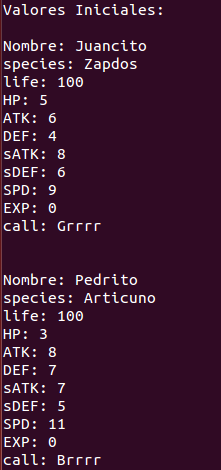
\includegraphics[scale=0.4]{estr1.png}
\caption{Valores Iniciales}
\end{figure}

\begin{figure}[ht]
\centering
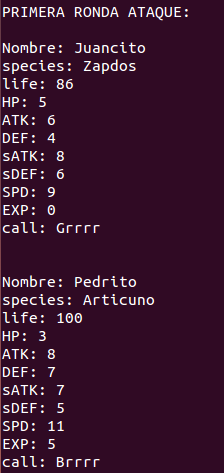
\includegraphics[scale=0.4]{estr2.png}
\caption{Primer Ataque}
\end{figure}

\begin{figure}[ht]
\centering
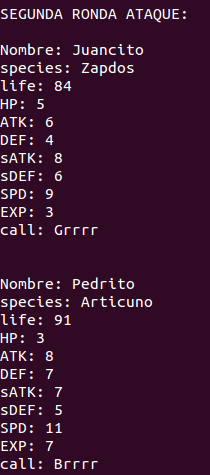
\includegraphics[scale=0.4]{estr3.png}
\caption{Segundo Ataque}
\end{figure}

Y así sucesivamente se desarrolla la batalla pokemon:

\end{document}